%%%%%%%%%%%%%%%%%%%%%%%%%%%%%%%%%%%%%%%
% Deedy - One Page Two Column Resume
% LaTeX Template
% Version 1.2 (16/9/2014)
%
% Original author:
% Debarghya Das (http://debarghyadas.com)
%
% Original repository:
% https://github.com/deedydas/Deedy-Resume
%
% IMPORTANT: THIS TEMPLATE NEEDS TO BE COMPILED WITH XeLaTeX
%
% This template uses several fonts not included with Windows/Linux by
% default. If you get compilation errors saying a font is missing, find the line
% on which the font is used and either change it to a font included with your
% operating system or comment the line out to use the default font.
% 
%%%%%%%%%%%%%%%%%%%%%%%%%%%%%%%%%%%%%%
% 
% TODO:
% 1. Integrate biber/bibtex for article citation under publications.
% 2. Figure out a smoother way for the document to flow onto the next page.
% 3. Add styling information for a "Projects/Hacks" section.
% 4. Add location/address information
% 5. Merge OpenFont and MacFonts as a single sty with options.
% 
%%%%%%%%%%%%%%%%%%%%%%%%%%%%%%%%%%%%%%
%
% CHANGELOG:
% v1.1:
% 1. Fixed several compilation bugs with \renewcommand
% 2. Got Open-source fonts (Windows/Linux support)
% 3. Added Last Updated
% 4. Move Title styling into .sty
% 5. Commented .sty file.
%
%%%%%%%%%%%%%%%%%%%%%%%%%%%%%%%%%%%%%%%
%
% Known Issues:
% 1. Overflows onto second page if any column's contents are more than the
% vertical limit
% 2. Hacky space on the first bullet point on the second column.
%
%%%%%%%%%%%%%%%%%%%%%%%%%%%%%%%%%%%%%%


\documentclass[]{deedy-resume-openfont}
\usepackage{fancyhdr}
\usepackage{tikzpagenodes}
 
\pagestyle{fancy}
\fancyhf{}
 
\begin{document}

%%%%%%%%%%%%%%%%%%%%%%%%%%%%%%%%%%%%%%
%
%     LAST UPDATED DATE
%
%%%%%%%%%%%%%%%%%%%%%%%%%%%%%%%%%%%%%%
%\lastupdated

%%%%%%%%%%%%%%%%%%%%%%%%%%%%%%%%%%%%%%
%
%     TITLE NAME
%
%%%%%%%%%%%%%%%%%%%%%%%%%%%%%%%%%%%%%%

\begin{tikzpicture}[remember picture,overlay,shift={(current page.north west)}]
\node[anchor=north west,xshift=1.75cm,yshift=-0.05cm]{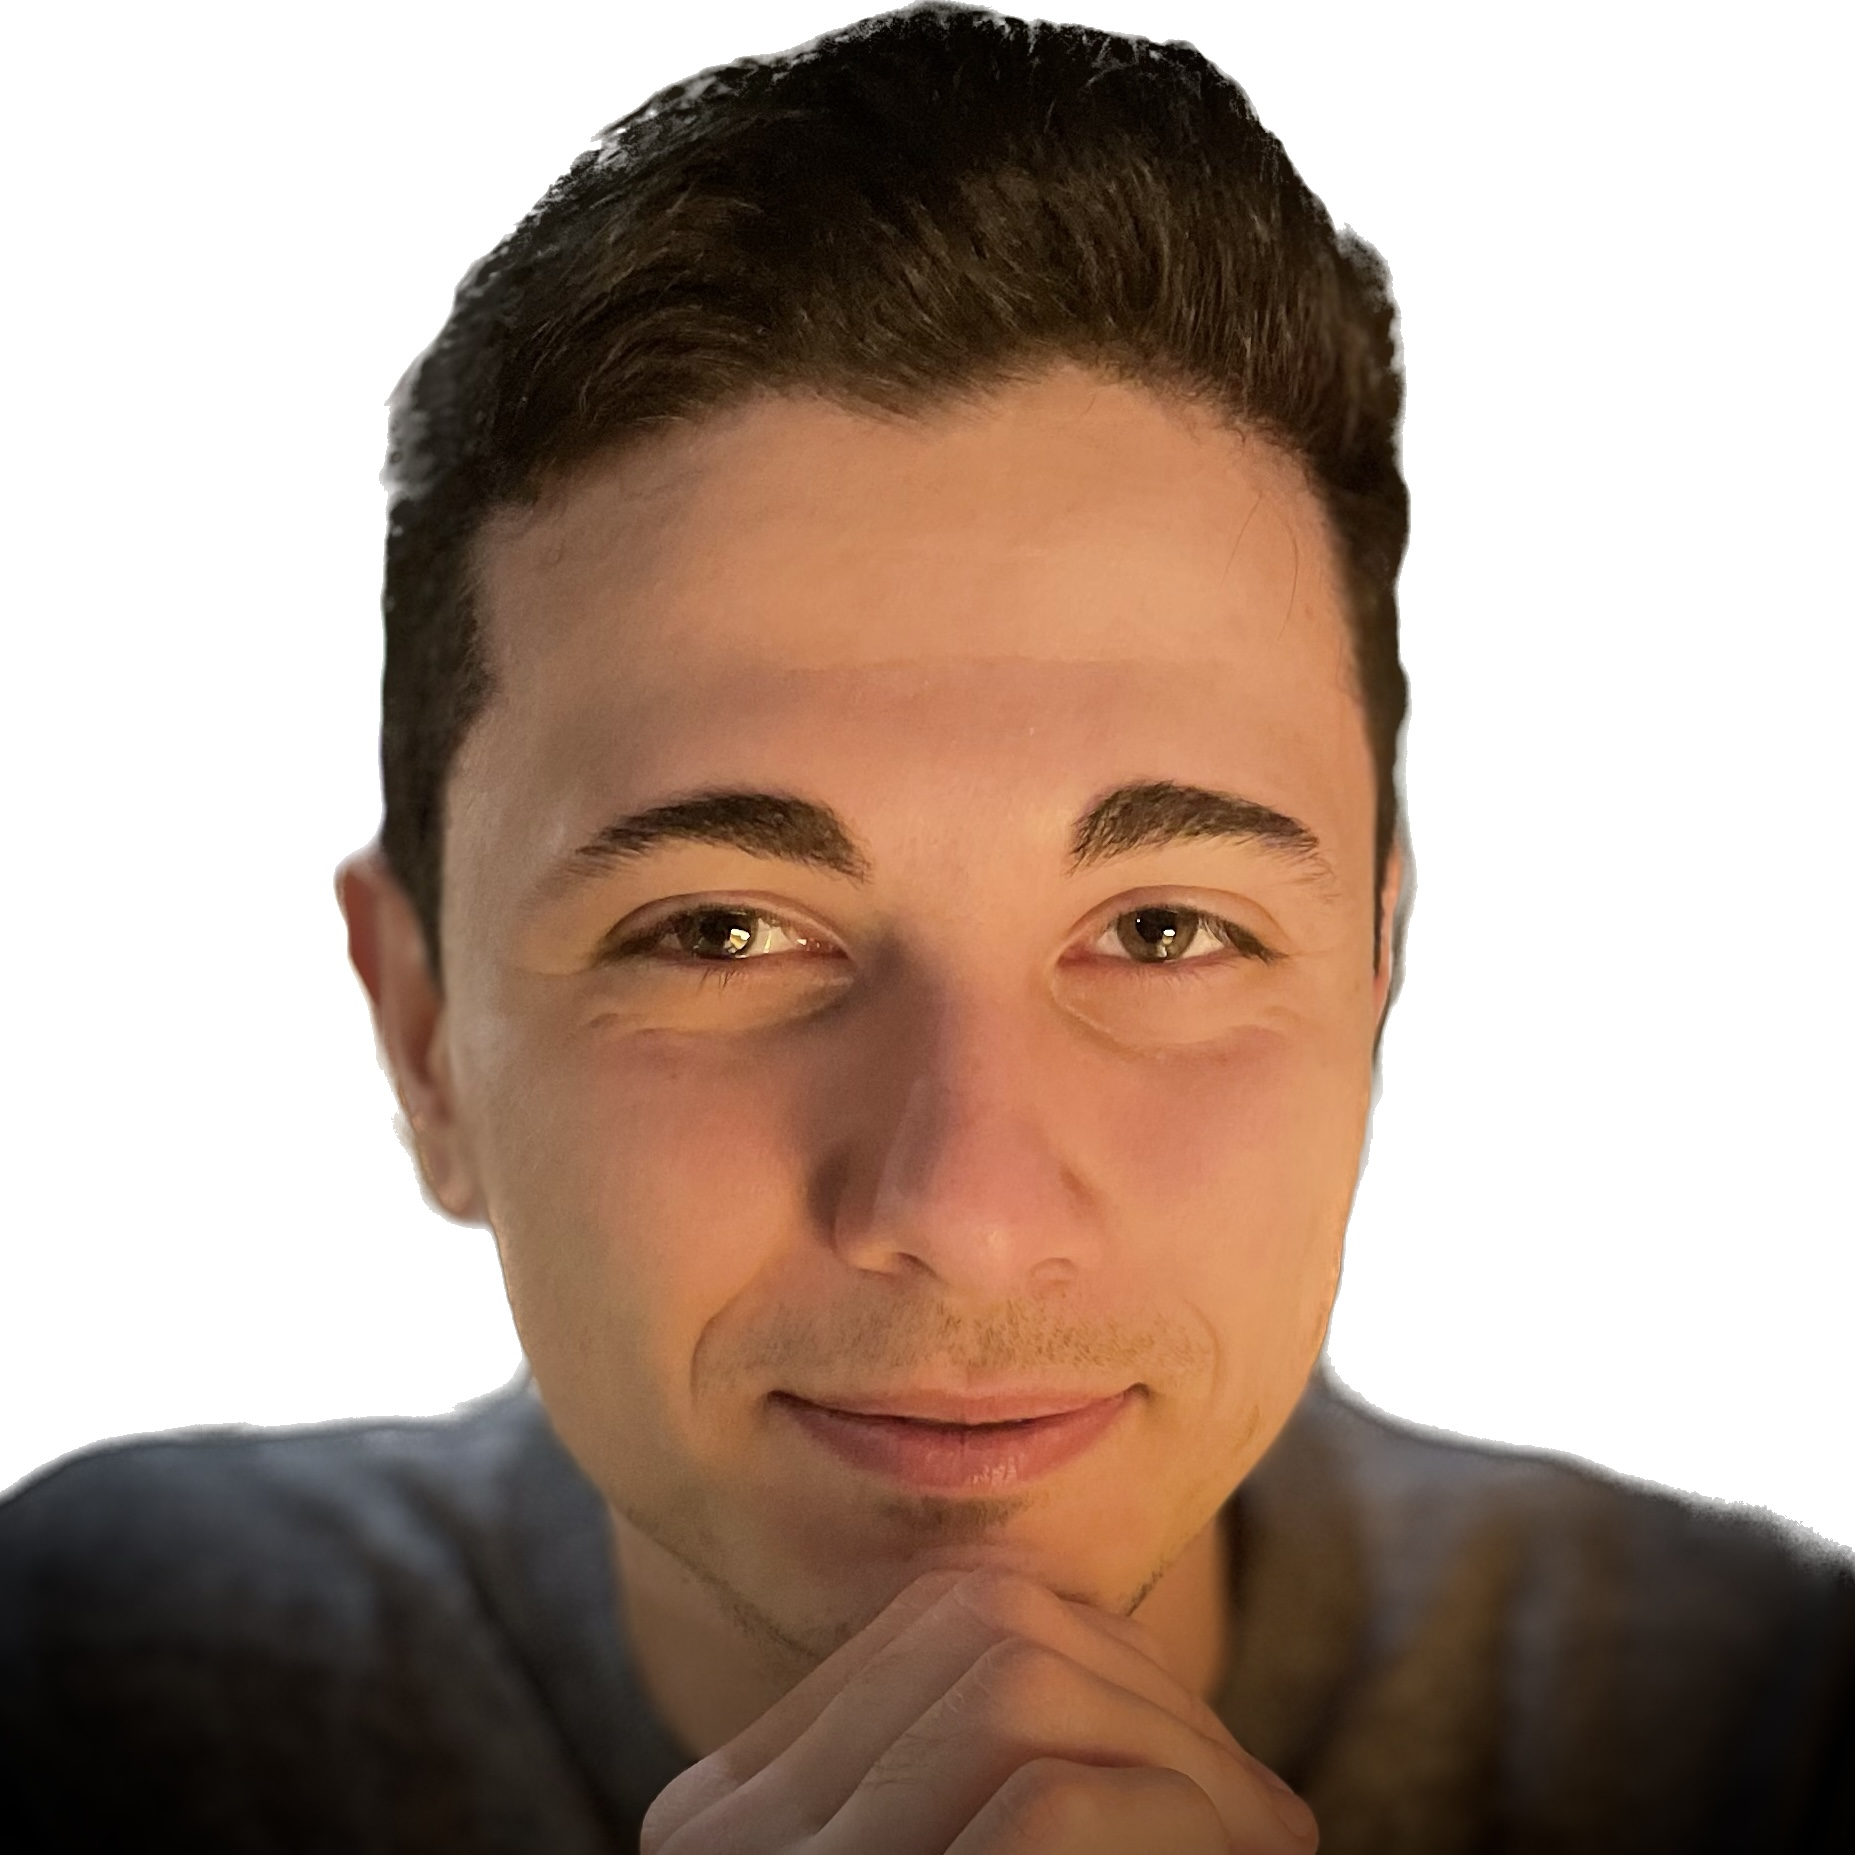
\includegraphics[width=2.25cm]{Foto.jpeg}};
\end{tikzpicture}

\namesection{Massimiliano}{Bruni}{
Email: \href{mailto:massimiliano.bruni@icloud.com}{massimiliano.bruni@icloud.com} | Mobile: 334 924 0665
}

%%%%%%%%%%%%%%%%%%%%%%%%%%%%%%%%%%%%%%
%
%     COLUMN ONE
%
%%%%%%%%%%%%%%%%%%%%%%%%%%%%%%%%%%%%%%

\begin{minipage}[t]{0.33\textwidth} 

%%%%%%%%%%%%%%%%%%%%%%%%%%%%%%%%%%%%%%
%     Profilo
%%%%%%%%%%%%%%%%%%%%%%%%%%%%%%%%%%%%%%

\section{Profile}
I am a Software Engineer specialized in Machine Learning. During my career I have realized and put into production various projects, both proprietaries and Open Source. I love technology and I like working on innovative projects. I work methodically, precisely and with attention to details. I am rational, diligent, hard-working and pragmatic.

%%%%%%%%%%%%%%%%%%%%%%%%%%%%%%%%%%%%%%
%     Link
%%%%%%%%%%%%%%%%%%%%%%%%%%%%%%%%%%%%%%

\section{Links} 
Github://\href{https://github.com/Maxinho96}{\bf Maxinho96} \\
LinkedIn://\href{https://www.linkedin.com/in/massimiliano-bruni-352926120}{\bf Massimiliano Bruni} \\
YouTube://\href{https://www.youtube.com/channel/UCqskrALDsaUvYC8ztJyqCug}{\bf Massimiliano Bruni}
\sectionsep

%%%%%%%%%%%%%%%%%%%%%%%%%%%%%%%%%%%%%%
%     Lingue
%%%%%%%%%%%%%%%%%%%%%%%%%%%%%%%%%%%%%%

\section{Languages}
\textbf{Italian}: Native \\
\textbf{English}: Upper-intermediate level B2/C1
\sectionsep

%%%%%%%%%%%%%%%%%%%%%%%%%%%%%%%%%%%%%%
%     Competenze
%%%%%%%%%%%%%%%%%%%%%%%%%%%%%%%%%%%%%%

\section{Skills}

\subsection{Hard Skills}
\textbf{Advanced:} Python \textbullet{} Machine Learning \textbullet{} NLP \\
Huggingface Transformers \textbullet{} Rasa Chatbot \\
FastAPI \textbullet{} Flask \textbullet{} Bash \textbullet{} Linux \textbullet{} Docker \\
Kubernetes \textbullet{} Git \\
\textbf{Intermediate:} Java \textbullet{} SQL \textbullet{} Elasticsearch \\
Matplotlib \textbullet{} NumPy \textbullet{} Pandas \textbullet{} macOS \\
\textbf{Basic:} Keras \textbullet{} TensorFlow \textbullet{} Scikit-learn \\
OpenCV \textbullet{} AWS \textbullet{} Hadoop \textbullet{} Spark \textbullet{} Golang
\sectionsep

\subsection{Soft Skills}
\textbf{Problem solving}, thanks to the Engineering studies. \\
\textbf{Team working}, thanks to the projects in which I was involved. \\
\textbf{Communication}, thanks to the experiences as private tutor and library assistant. \\
\textbf{Learning}, thanks to my passion for understanding the world.

%%%%%%%%%%%%%%%%%%%%%%%%%%%%%%%%%%%%%%
%     Esami rilevanti
%%%%%%%%%%%%%%%%%%%%%%%%%%%%%%%%%%%%%%

% \section{Esami rilevanti}
% \textbf{Intelligenza Artificiale}: 30 e lode \\
% \textbf{Machine Learning}: 30 e lode \\
% \textbf{Sistemi Intelligenti per Internet}: 30 e lode \\
% \textbf{Big Data}: 28 \\
% \textbf{Analisi e Gestione dell'informazione su web}: 30
% \sectionsep

%%%%%%%%%%%%%%%%%%%%%%%%%%%%%%%%%%%%%%
%     Certificazioni
%%%%%%%%%%%%%%%%%%%%%%%%%%%%%%%%%%%%%%

\section{Certifications}
\begin{tabular}{@{}lll@{}}
\textbf{Year} & \textbf{Released by} & \textbf{Certificate} \\
2022          & B9lab         & \textit{Interchain Developer} \\
              &               & \textit{Academy} \\
2022          & Rasa chatbot  & \textit{Rasa Developer} \\
              &               & \textit{Certification} \\
2021          & Coursera      & \textit{Deep Learning} \\
              &               & \textit{Specialization} \\
2020          & Italian State & \textit{Software}\\
              &               & \textit{Engineering License} \\
2017          & Coursera      & \textit{Machine Learning} \\
2015	      & Cambridge     & \textit{B2 First} \\
2015	      & Cisco         & \textit{CCNA Discovery} \\
\end{tabular}
\sectionsep

%%%%%%%%%%%%%%%%%%%%%%%%%%%%%%%%%%%%%%
%     Hobby
%%%%%%%%%%%%%%%%%%%%%%%%%%%%%%%%%%%%%%

\section{Hobbies}
Sports \textbullet{} Technology news \textbullet{} Videogames \\
Board games \textbullet{} Mangas \textbullet{} Hangout

%%%%%%%%%%%%%%%%%%%%%%%%%%%%%%%%%%%%%%
%
%     COLUMN TWO
%
%%%%%%%%%%%%%%%%%%%%%%%%%%%%%%%%%%%%%%

\end{minipage}
\hfill
\begin{minipage}[t]{0.66\textwidth} 

%%%%%%%%%%%%%%%%%%%%%%%%%%%%%%%%%%%%%%
%     Esperienze
%%%%%%%%%%%%%%%%%%%%%%%%%%%%%%%%%%%%%%

\section{Experience}

\subsection{HCL Software}
\descript{Software Engineer - Machine Learning}
\location{May 2021 - present | Rome}
I am responsible of developing the Python backend and the training process of new projects that require Machine Learning. I am also involved in the product delivery process in both cloud and on-premise environments. \\
Technologies: \textbf{Python} \textbullet{} \textbf{Pandas} \textbullet{} \textbf{Huggingface} \textbullet{} \textbf{Rasa} \textbullet{} \textbf{FastAPI} \textbullet{} \textbf{Bash} \textbullet{} \textbf{Docker} \textbullet{} \textbf{Kubernetes} \textbullet{} \textbf{Elasticsearch}
\sectionsep

\subsection{Askdata}
\descript{Machine Learning Engineer}
\location{September 2020 - April 2021 | Rome}
I was responsible of R\&D and releasing in production Deep Learning models in the NLP field involving Text Summarization, Machine Translation, Named Entity Recognition and Semantic Similarity. \\
Technologies: \textbf{Python} \textbullet{} \textbf{Pandas} \textbullet{} \textbf{Huggingface} \textbullet{} \textbf{SpaCy} \textbullet{} \textbf{Flask} \textbullet{} \textbf{FastAPI}
\sectionsep

\subsection{Italian Research Center (CNR)}
\descript{Internship in Machine Learning and Computer Vision}
\location{March 2018 - July 2018 | Rome}
Internship for the Bachelor's thesis, where I developed the project called \textit{Object recognition robot}, linked below. \\
Technologies: \textbf{Python} \textbullet{} \textbf{TensorFlow} \textbullet{} \textbf{Scikit-learn} \textbullet{} \textbf{OpenCV} \textbullet{} \textbf{Matplotlib} \textbullet{} \textbf{Numpy}


%%%%%%%%%%%%%%%%%%%%%%%%%%%%%%%%%%%%%%
%     Istruzione
%%%%%%%%%%%%%%%%%%%%%%%%%%%%%%%%%%%%%%

\section{Education} 

\subsection{Università degli Studi Roma Tre}
\descript{Master's Degree in Computer Science Engineering}
\location{October 2018 - July 2020 | Rome}
\location{Grade: 110/110 cum laude}
\sectionsep

\subsection{ITALIAN RESEARCH CENTER (CNR)}
\descript{Advanced School in Artificial Intelligence}
Practical school with focus on Machine Learning Applications. \\
\location{October 2019 - April 2020 | Rome}
\sectionsep

\subsection{Università degli Studi Roma Tre}
\descript{Bachelor's Degree in Computer Science Engineering}
\location{September 2015 - July 2018 | Rome}
\location{Grade: 110/110 cum laude}


%%%%%%%%%%%%%%%%%%%%%%%%%%%%%%%%%%%%%%
%     Progetti
%%%%%%%%%%%%%%%%%%%%%%%%%%%%%%%%%%%%%%

\section{Projects}

\descript{Clara (\href{https://www.hcltechsw.com/clara}{Link})}
A chatbot virtual assistant for Workload Automation.

\descript{AI Data Advisor (\href{https://youtu.be/TAksOKMvM48}{Link})}
An Anomaly Detection System for Workload Automation.

\descript{Human2SQL (\href{https://www.askdata.com/product}{Link})}
Translation from spoken language to SQL language.

\descript{Video surveillance system (\href{https://github.com/Maxinho96/person\_identification}{Link})}

\descript{Object Detection with drone (\href{https://youtu.be/cnnGjHns818}{Link})}

\descript{Telegram bot: Image Classifier (\href{https://github.com/Maxinho96/Image-Classifier-Telegram-Bot}{Link})}

\descript{Object recognition robot (\href{https://github.com/Maxinho96/Machine-Learning-Research-Project}{Link})}

\section{Open Source contributions}

\descript{Rasa chatbot framework (\href{https://github.com/RasaHQ/rasa/pulls?q=is\%3Apr+author\%3AMaxinho96}{Link})}

\descript{Huggingface Transformers (\href{https://github.com/huggingface/transformers/pulls?q=is\%3Apr+author\%3AMaxinho96}{Link})}

\descript{YOLOv3 Tensorflow implementation (\href{https://github.com/zzh8829/yolov3-tf2/pulls?q=is\%3Apr+author\%3AMaxinho96}{Link})}

%%%%%%%%%%%%%%%%%%%%%%%%%%%%%%%%%%%%%%
%     Dati personali
%%%%%%%%%%%%%%%%%%%%%%%%%%%%%%%%%%%%%%

\footnotetext{I authorize to use and process my personal details contained in this document.}

\end{minipage} 
\end{document}  \documentclass[]{article}
